%% ============================================================
%%  Chapter 4 - Conception of the Proposed System
%%  Raw commands/configs deferred to
%%  Chapter 5 and the annexes, per the template rule.
%%  Only external citation needed here: sharafaldin2018cicids.
%% ============================================================

\chapter{Conception of the Proposed System}
\label{chap:conception}

\section{Introduction}
\label{sec:conception_intro}

I finished up the last chapter highlighting four areas in which the existing intrusion detection landscape left something to be desired. In fact, the entire design of this project revolves around those very areas: that this project must detect attacks that it has not explicitly been coded for (Gap~1), that it will be deployed in a private cloud using commodity hardware and will not be reliant upon a commercial provider platform (Gap~2), that this project must present understandable reasons for its alerts to users, not simply identify threats as they occur (Gap~3) and that the solution will operate in a low-latency, time-constrained environment handling live traffic rather than offline, batch processing of historical data (Gap~4).

The following chapter describes how those four requirements lead to a real-world design, covering: the overall architecture of the system, the decision to model a real-world private cloud using a virtual two-machine lab, the justifications for key environmental decisions, the dataset, the approach to the dataset's features, and the method of training and choosing a detection model. The focus of this chapter is primarily \emph{what} we decided to build and \emph{why}. The building itself the exact commands, the configuration files, and screen captures of the system running  together with its measured outcomes, will be addressed in Chapter~\ref{chap:results}. Where choices involved tradeoffs, alternative directions which were not taken are also described, for the alternative paths in a project such as this are generally as informative as the successful one.

% ─────────────────────────────────────────────────────────────
\section{Overall Architecture}
\label{sec:conception_architecture}

At the highest level the system is a pipeline of four stages, each feeding the next. Traffic is \textbf{captured} from the network, converted into \textbf{flow features}, passed to a \textbf{detection} model, and any alert is then \textbf{explained and surfaced} to an analyst. Figure~\ref{fig:architecture} shows the arrangement.

\begin{figure}[H]
  \centering
  \IfFileExists{figures/system_architecture.png}{%
    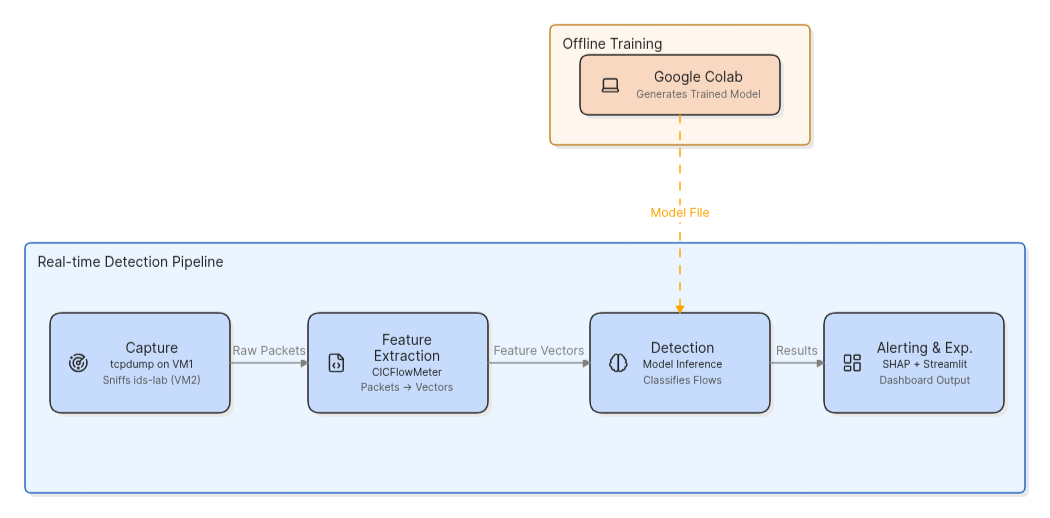
\includegraphics[width=0.92\textwidth]{figures/system_architecture.png}%
  }{%
    \fbox{\parbox{0.85\textwidth}{\centering\vspace{1.2cm}
    \texttt{[Figure: system\_architecture.png  to be created]}\\[4pt]
    \small Original block diagram of the four-stage pipeline. Left to right:
    (1)~\textbf{Capture}  attack traffic from VM2 crossing the \texttt{ids-lab}
    network, sniffed by \texttt{tcpdump} on VM1; (2)~\textbf{Feature extraction}
     CICFlowMeter turning packets into flow feature vectors;
    (3)~\textbf{Detection}  the trained model classifying each flow;
    (4)~\textbf{Alerting \& explanation}  SHAP annotating the alert, intended
    for presentation on an analyst dashboard. A separate offline box (Google Colab) feeds a single
    \emph{trained model} arrow into the detection stage, to show that training
    happens outside the lab and only the resulting model is deployed. Draw in
    draw.io or PowerPoint.
    \vspace{1.2cm}}}%
  }
  \caption{Four stage architecture of the proposed IDS}
  \label{fig:architecture}
\end{figure}

Two of the points illustrated in the diagram were design decisions themselves, not mere details. One is that the detector lives on the same physical machine as the service it protects. This is VM1 in our lab setup and it was intentionally chosen to serve a double purpose: It houses the legitimate, target services that get attacked and it also hosts the detector that is watching them. 
It's how the IDS operates in a real deployment, either it runs on the system or just next to it.

As we saw in the "cloud blind spot" discussed in Chapter~\ref{chap:cloud}, the east-west traffic that typically goes unnoticed is in fact inspected by our detector because it is running on the machine the traffic hits first. The second design point is that the training occurs off-line and apart from the pipeline. The model is not trained on VM1. Instead, it is built and completed at a later point and then simply supplied to the detector part as a fixed entity. 
Section~\ref{sec:conception_training} explains why, but it's worth reasserting the effect of the choice in architecture. 
Our deployed system trains only as an afterthought. When it's "live", it simply loads a previously trained model and inspects traffic. This makes it possible to run an already wellperforming detector on the relatively constrained lab VM and keeps the concerns of model building separate from those of running and deploying a detector.
% ─────────────────────────────────────────────────────────────
\section{Environment Design Decisions}
\label{sec:conception_environment}

The project aim given is an IDS for organisations on a private cloud, and the most loyal target environment is therefore the true private cloud equivalent, OpenStack. This was rejected, for the following reasons and I thought they warranted inclusion as they are the context for the rest of the story.

\subsection{A simulated cloud rather than OpenStack}
\label{sec:conception_nostack}

There are three reasons this work doesn't build on top of OpenStack. The first is hardware: even a small, stable deployment of OpenStack needs at minimum a dedicated server with far more memory than my laptop has; running the OpenStack control plane and the development tools on the same 16~GB laptop is a completely impractical proposition. The second is complexity and brittleness: OpenStack is roughly 15 interdependent services; installations from scratch take multiple days and are extremely brittle when it comes to upgrades not a worthwhile investment for a project whose actual innovation lies elsewhere.
The third reason follows from the second: the research value added here is the explanatory pipeline itself, and any effort devoted to wrangling OpenStack infrastructure isn't devoted to the actual detector and its explanations.

So the better strategy is to develop and test the proposed IDS on an isolated, emulated network that mimics a private cloud, where the only traffic is that between the guest VMs over KVM, rather than taking on the management of a real and complex platform. What is crucial to an IDS is the network traffic it sees, and that traffic is faithfully reproduced here. A future deployment on a real OpenStack setup is noted as an extension.

\subsection{Two real machines rather than a network emulator}
\label{sec:conception_twovms}

Another possibility, other than two separate virtual machines, would have been using a network emulator, like Mininet, inside a single virtual machine and scripting both the attacker and victim as emulated nodes. However, this idea was rejected, mainly because of one main reason and two other supporting ones.

Why is real traffic production the killer feature?
A real attack tool performing SSH brute forcing on a real SSH server sends actual TCP handshake packets with genuine timing, as well as real authentication packets, as opposed to simply using the packet-level flow characteristics that an emulator will fake. The reason that the entire thing hangs together logically, is that the features generated byCICFlowMeter on the actual traffic are of the exact same type as those contained in CICIDS-2017, because that dataset was generated by using the very same attack tool on actual services. 
If you try this with an emulated flow set, your resulting features will have a completely different distribution, and your detection algorithm will be assessing something other than the patterns it was trained to detect. 
In essence, feature comparability between the data you're trying to detect and the training data is the glue holding this whole detection exercise together, and only real traffic achieves that. There are two minor reasons to run the whole thing on two actual machines. Firstly, it is how real world IDS deployments are situated (usually close to the systems that they defend). Secondly, running the detection engine on one box, while launching the attacks on another actually provides a much better live demo (an attack running on screen A, with an alert popping up on screen B) than can be achieved with just repeating packets.

\subsection{KVM rather than VirtualBox}
\label{sec:conception_kvm}

Since the host machine is running a Linux operating system, the “native” hypervisor is the built in Linux kernel facility of KVM, not an installable, user space product like VirtualBox. For a Linux host KVM has the added benefits that virtualised instructions are processed by the kernel directly, no intervening user space process to translate to their native performance network interface, \texttt{virtio}, makes close to line speed possible which is relevant since our goal is the packets themselves and their \texttt{qcow2} disks are thinly provisioned, growing as they’re written rather than preallocating the full disk space. Given the goal, for traffic capture on a Linux laptop, there’s only one real candidate.

% ─────────────────────────────────────────────────────────────
\section{Virtual Machine and Network Design}
\label{sec:conception_vmnet}

The laboratory is two virtual machines on an isolated network, each of which has an asymmetric role: one is the victim and the other, a purely offensive machine. \textbf{VM1}, powered by Ubuntu Server, plays the dual role of target and detector. Hence, it has more responsibility than VM2, having been allotted 5 GB of RAM, four virtual cores and a 35 GB thin provisioned hard disk space. The memory requirement was calculated as sum of maximum possible usage by pipeline components: operating system, container runner, streaming broker, attack detector, tracker \& dashboard service, database \& CICFlowMeter java heap, which reached up to 3.6GB under stress. 
A larger portion has been assigned to prevent memory overflow from the streaming broker, during a live demonstration. 

More details can be found in table \ref{tab:vm1_ram}. Two more CPUcores are given to avoid possible bottlenecks as CICFlowMeter is Java process that demands significant resources while streaming broker uses all available cores. Ubuntu Server edition, in head less format, has been utilized for this server, since graphical environments would have consumed precious memory resources needed for running containers and real production servers are typically head less.

\begin{table}[H]
  \centering
  \caption{VM1 peak memory budget under sustained attack simulation.}
  \label{tab:vm1_ram}
  \renewcommand{\arraystretch}{1.3}
  \begin{tabular}{lr}
    \toprule
    \textbf{Component} & \textbf{Approx. peak (MB)} \\
    \midrule
    Ubuntu Server (base OS)      & 400 \\
    Container runtime            & 200 \\
    Streaming broker + coordinator & 800 \\
    Detection engine             & 400 \\
    Experiment tracking service  & 300 \\
    Dashboard                    & 300 \\
    Database                     & 200 \\
    CICFlowMeter (Java heap)     & 512 \\
    System buffers               & 500 \\
    \midrule
    \textbf{Total peak}          & \textbf{$\approx$3\,600} \\
    \textbf{Allocated}           & \textbf{5\,120 (5\,GB)} \\
    \bottomrule
  \end{tabular}
\end{table}

\textbf{VM2} is the attacker machine and needs much less. It is a standard lightweight desktop, using a penetration testing distribution. The vm was allocated 3~GB of RAM, two vCPUs, and a 30~GB disk. 
We chose this distribution because the desired penetration testing tools (which were used to perform the brute force, flood, scan, exploitation and packet capture steps) came installed and are actively maintained; not doing this would require another 5-7 days of tool installation. 
We opted for a lightweight desktop because, at the given RAM allocation, this difference was substantial.

The two VMs are connected to each other on an \textbf{isolated internal network} (\texttt{ids-lab} network, operating on a dedicated private subnet) and they exchange nothing else but traffic used for the purposes of this study (both attacker and detector traffic). We chose isolation, to prevent noise from other network activities from interfering with detection. An additional network interface on each of the two VMS connected to standard NATed network for accessing to the internet and performing operations like packages installation and update; this one does not carry project traffic. 
This distinction parallels the north-south vs. east-west distinction in the cloud as introduced in chapter~\ref{chap:cloud}; in fact, NAT connection represents the north-south path and the \texttt{ids-lab} network represents the east-west path monitored by the detector. 
We had to work around a minor issue in routes configurations, in order to force the NAT interface to serve as default route, as explained in chapter~5.

% ─────────────────────────────────────────────────────────────
\section{Dataset and Feature Strategy}
\label{sec:conception_dataset}

For learning based detector requires some data that is labeled so that it could learn from it, thus what kind of things to learn it depends on what data is used. This project is concerned with CICIDS-2017 \cite{sharafaldin2018cicids}, and is selected for three reasons. First is its realism; the data was collected over 5 days from simulated users in order to create a similar texture to the network data that this system receives in production as it utilizes real protocols and is not generated using synthetic packet generation. 
Second is coverage of the different attacks that this project stages in the laboratory: namely port scan, brute force attack, web attack, denial of service. 
Third, is feature format; this feature files were created using CICFlowMeter which is also the same tool that the production pipeline uses for this purpose, thus data is in same representation for both training and testing data, and that is the only thing needed to successfully deploy models trained in one in another environment.
The data come in the form of raw packets and feature file set. Only feature file set are needed as raw data have already converted into the given feature files, thus no point for conversion again, it only will reproduce the same data set, so what is important here is just a set of feature files. From 5 days of the data, 2 days are omitted and some of days selected are as in Table. \ref{tab:dataset_days}. 

From all days, we are keeping days of pure benign traffic as a base line of normal traffic,brut force attack day, denial of service day, port scan attack day, and web attack day as this attacks we are implementing in the lab. 
We also include the distributed denial of service day to differentiate from brute force attack. We are excluding 2 days from 5 days data: one of infiltration days and one of botnet days; these two days had relatively less data as well as both attack categories were typically dropped or reported with almost zero accuracy in the research literature; including them would therefore just increase imbalance without significantly impacting the data quality. In fact class imbalance itself is another issue, which was pointed out in the preceding section regarding misleading use of the accuracy alone; this concern impacts the selection of performance evaluation metrics as described below.

\begin{table}[H]
  \centering
  \caption{CICIDS-2017 days selected for training, with rationale.}
  \label{tab:dataset_days}
  \renewcommand{\arraystretch}{1.3}
  \begin{tabularx}{\textwidth}{llX}
    \toprule
    \textbf{Day (traffic)} & \textbf{Decision} & \textbf{Reason} \\
    \midrule
    Monday (benign)          & Keep & The only purely benign day; baseline of normal traffic \\
    Tuesday (brute force)    & Keep & SSH/FTP brute force matches the lab attacks \\
    Wednesday (DoS)          & Keep & Several denial-of-service variants \\
    Thursday AM (web)        & Keep & Web attacks against a web server, as in the lab \\
    Thursday PM (infiltration) & Drop & Very few samples; complex multi stage chain \\
    Friday AM (port scan)    & Keep & Scanning matches the lab attacks \\
    Friday PM (DDoS)         & Keep & Distinct from single source flooding \\
    Friday PM (botnet)       & Drop & Extremely few samples; severe imbalance \\
    \bottomrule
  \end{tabularx}
\end{table}

% ─────────────────────────────────────────────────────────────
\section{Detection Model and Training Methodology}
\label{sec:conception_training}

This classifier in the center of the pipeline is a supervised learning algorithm which has been trained on the training data as defined previously. The algorithm to use is not pre-determined; multiple classification candidates have been trained, and the best one selected, as Chapter~\ref{chap:ai} gives arguments for the answer being unexpected.

\subsection{Candidate models}
\label{sec:conception_candidates}

Three models are trained as candidates. A Random Forest as a baseline, because as argued in Section~\ref{sec:classical_ml}, they're fast to train, fast to infer, intrinsically interpretable, and frequently compete in accuracy with more cumbersome models on flow level features. Training a pair of deep models   a convolutional network and an LSTM   for as discussed in Chapter~\ref{chap:ai}, slow scans in particular put their signature into the ordering of packets, a sequence model should capture. By comparing all three, we move the classical vs deep debate of Chapter~\ref{chap:ai} from abstract to concrete, on data for the task.

\subsection{Training offline, deploying the result}
\label{sec:conception_offline}

We do the training offline, on Google Colab, isolated from the lab. That is intentional and on three counts. It leaves the computationally expensive, memory expensive data pre-processing and model training on the machine not in the development room, thus preventing any crashes that come from trying to train enormous models locally. 
It offers us the ability to use a good, free GPU for the deepest models. 
And it make training repeatable and portable the notebook contains everything anyone can re execute. A nice, clean separation of duties is then the result: producing a good model is an offline task, and using that good model is an in lab online task.

\subsection{How the models are judged}
\label{sec:conception_metrics}

The class imbalance poses a problem to accuracy because the large proportion of normal traffic means that simply outputting benign as always yields high accuracy, but catches none, just as the problem raised in Section~\ref{sec:classical_ml} has done. We therefore focus instead on the precision, recall and the F1-score, which behave appropriately in imbalanced data. The penalty for missing attacks should be high for a detector so the recall metric is prioritized above the precision, though we again acknowledge the trade off. 
All results are logged using a centralised experiment tracking system so that we are not relying on human memory when comparing competing candidate models. 
The resulting comparison is provided in Chapter~\ref{chap:results}.

% ─────────────────────────────────────────────────────────────
\section{Real Time Detection and Explainability}
\label{sec:conception_realtime}

The last two steps of the pipeline serve to distinguish our system from a model that simply scores a static file. And indeed they answer the last two gaps identified in Chapter~\ref{chap:ids} directly. In the \textbf{liveness} design, the model is intended to sit behind a streaming component.

The design intercepts traffic, transforms it into flow features, then publishes them on a message broker to a detection service, which would inspect and classify each flow as it arrives rather than running on a static batch.

A data path of this shape is what allows an intrusion detector to cope with the strict time constraints imposed by live traffic, addressing the motivation behind Gap~4. The present work implements and validates the detection core offline; the streaming deployment, including the concrete choice of broker, is specified here as a design and left as future work, revisited in the discussion of Chapter~\ref{chap:results}. As for \textbf{explainability}, any alert is pushed through a SHAP explainer before it can be consumed by an analyst. Our detector alone only states that an alert is an attack, whereas the SHAP explainer highlights which features were responsible for this verdict  an unusually high number of half open connection, a shorter than usual flow, etc. This process gives the analyst the reason behind the attack, transforming an opaque detection into actionable insight, i.e., a verdict an analyst can use to block traffic, to escalate an incident, or even to dismiss the alert as a false positive when the justification is provided. 

In the intended production interface, the analyst interacts with the system through a dashboard where these explained alerts are presented. Chapter~\ref{chap:results} applies the SHAP layer to the trained detector directly; the analyst facing dashboard is described as the target interface and left as future work.
% ─────────────────────────────────────────────────────────────
\section{Summary}
\label{sec:conception_summary}

The design replaces the four separate gaps described in the last chapter by one integrated pipeline. An algorithmically driven detector is used to detect novel attacks, a virtualised 2 machine environment hosted by a KVM hypervisor provides an abstraction of a private cloud, enabling the design to be tested with the intention of running on commodity hardware, a SHAP layer is placed in line with each alert to assist with explainability and the entire pipeline is designed to run as a streaming job for liveness. We make the choices on environment (both for realistic traffic and to reduce our focus away from cloud plumbing and onto our detection system), data (to make the model train and operate on the same feature set) and our offline experiment process (to enable evaluation against 3 alternatives before deploying our strongest to the lab) to minimise external sources of variation from the evaluated model. We present here only the design and justification: Chapter~\ref{chap:results} implements the detection core and evaluates its effectiveness, both on the CICIDS-2017 benchmark and on attack traffic generated independently in the lab.
